\section{Week 4: Learning to Rank (LTR) and Interactions}

\subsection{Preliminaries and Goal} 

\textbf{Representation}: \\
Represent the document and query in a format that a ML model can use: \textcolor{Maroon}{a numerical vector} $\vec{x} \in \mathbb{R}^{n}$.\\
\\
\textbf{Prediction}: \\
Then a \textcolor{Maroon}{ranking model} $f : \vec{x} \rightarrow \mathbb{R}$ is optimized to score each document-query combination so that relevant documents are scored higher. \\
In mathematical terms: $f$ maps a vector to a real-valued score. \\
\\
\textbf{Features}: \\
Traditionally features are hand-crafted to encode IR insights, nowadays we also have \textit{\textcolor{MidnightBlue}{deep learned}} features. \\
\\
They can be categorized as: 
\begin{itemize}
    \setlength\itemsep{0em}
    \item \textbf{\textcolor{Maroon}{Document-only}} or static features (e.g., document length)
    \item \textbf{\textcolor{Maroon}{Document-Query-combination}} or dynamic features (e.g., BM25)
    \item \textbf{\textcolor{Maroon}{Query-only}} features (e.g., query length)
\end{itemize}

\newpage
\textbf{Models can be trained on different data}:
\begin{itemize}
    \setlength\itemsep{0em}
    \item \textbf{\textcolor{Maroon}{Offline or Supervised}} LTR: learn from annotated data.
    \begin{itemize}
    \setlength\itemsep{0em}
        \item Expensive and time consuming.
        \item Provides ground truth
    \end{itemize}
    \item \textbf{\textcolor{Maroon}{Online/Counterfactual}} LTR: learn from user interactions.
    \begin{itemize}
    \setlength\itemsep{0em}
        \item Virtually free and easy to obtain.
        Hard to interpret.
    \end{itemize}
\end{itemize}

\subsection{Offline LTR}
Data is obtained by:
\begin{enumerate}
\setlength\itemsep{0em}
    \item Pay some humans to be annotators (and train them to be good annotators).
    \item Collect a set of queries
    \item Preselect a large (not too large) set of documents per query.
    \item Show document-query pairs to annotators.
    \item Annotators rate every document-query pair on their relevance (e.g. on a scale from 0 to 4).
\end{enumerate}

\textbf{Goal}: \\
We have:
\begin{itemize}
\setlength\itemsep{0em}
    \item Feature representation of document-query pairs: $\vec{x}_{q,d} \in \mathbb{R}$.
    \item Labels indicating the relevance of document-query pairs: $y_{q,d} \in [0,4]$
\end{itemize}

And we want:
\begin{itemize}
\setlength\itemsep{0em}
    \item A function $f: \vec{x} \rightarrow \mathbb{R}$ that scores documents.
    \item To get the best ranking by sorting according to $f(\vec{x})$.
\end{itemize}

How to find $f$?

\subsection{Pointwise approach}
Regression-based or classification-based approaches are popular. \\
\\
\textbf{Regression loss}: \\
Given $\langle q, d\rangle$ predict the value of $y_{q,d}$. \\
\\
E.g., \textcolor{MidnightBlue}{square loss} for binary or categorical labels:
$$ \mathcal{L}_{\text {Squared }}\left(q, d, y_{q, d}\right)=\left\|y_{q, d}-f\left(\vec{x}_{q, d}\right)\right\|^{2} $$

where $y_{q,d}$ is the one-hot representation or the actual value of the label.

\textbf{Classification loss}: \\
Given $\langle q, d\rangle$ predict the class $y_{q,d}$. \\
\\
E.g., \textcolor{MidnightBlue}{Cross-Entropy} with \textcolor{MidnightBlue}{Softmax} over categorical labels $Y$:
$$ \mathcal{L}_{\mathrm{CE}}\left(q, d, y_{q, d}\right)=-\log \left(p\left(y_{q, d} \mid q, d\right)\right)=-\log \left(\frac{e^{\sigma \cdot s_{y_{q, d}}}}{\sum_{y \in Y} e^{\sigma \cdot s_{y}}}\right) $$

where $s_{y_{q, d}}$ is the model's score for label $y_{q,d}$.\\
\\
\textbf{\textcolor{Red}{Issues}} with \textbf{pointwise approaches}:
\begin{itemize}
\setlength\itemsep{0em}
    \item \textbf{Class imbalance}: many irrelevant documents and very few relevant documents.
    \item \textbf{Query level feature normalization needed}: distr. of features differs greatly per query
\end{itemize}

\textcolor{Maroon}{But}, these can be overcome. \\
\\

\textbf{The \textcolor{Red}{fundamentally wrong part} is}: \\
\textcolor{Maroon}{Ranking is not a regression or classification problem}. \\
\\
A document-level loss does not work for raking problems because document scores should not be considered independently (\textcolor{Maroon}{pointwise methods do not directly optimize ranking quality}). 
\subsection{Pairwise approach}
Instead of looking at document-level, consider \textcolor{MidnightBlue}{pairs of documents}. 
$$ P\left(d_{i} \succ d_{j}\right)=f\left(\vec{x}_{i}, \vec{x}_{j}\right) $$

Do \textcolor{Maroon}{not} change the model to take \textcolor{Maroon}{document pairs as input} (would be quadratic in complexity: $O\left(N^{2}\right)$, during \textcolor{Maroon}{inference}). \\
\\
The scoring model remains \textcolor{Maroon}{unchanged}: $f(\vec{x_i}) = s_i$, but the \textcolor{MidnightBlue}{loss function} is based on \textcolor{Maroon}{document pairs}:
$$ \mathcal{L}_{\text {pairwise }}=\sum_{d_{i} \succ d_{j}} \phi\left(s_{i}-s_{j}\right) $$

Thus we still score documents and then order according to scores.
\newpage
\textbf{\textcolor{Red}{Pairwise loss functions}}: \\
Pairwise loss minimizes the \textcolor{Maroon}{average number of inversions} in ranking: \\
$d_{i} \succ_{q} d_{j}$ but $d_{j}$ is ranked higher than $d_{i}$\\
\\
\textbf{Generally} the following form: 
\begin{equation*}
    \mathcal{L}_{\text {pairwise }}=\phi\left(s_{i}-s_{j}\right)
\end{equation*}

where $\phi$ can be:
\begin{itemize}
\setlength\itemsep{0em}
    \item \textbf{Hinge function}: $\phi(z) = \max(0, 1-z)$
    \item \textbf{Exponential function}: $\phi(z) = e^{-z}$
    \item \textbf{Logistic function}: $\phi(z) = \log(1 + e^{-z}$
    \item etc.
\end{itemize}
\vspace{0.5cm}
{\Large \textbf{\textcolor{NavyBlue}{RankNet}}} (using $\sigma$ instead of $\gamma$, following assignment notation): \\
is a pairwise loss function - popular choice for training neural LTR models. \\
\\
For a given query, each pair of documents $D_{i}$ and $D_{j}$ with differing labels is chosen, and each such pair (with feature vectors $x_{i}$ and $x_{j}$) is presented to the model, which computes the scores $s_{i}=f\left(x_{i}\right)$ and $s_{j}=f\left(x_{j}\right)$. Let $D_{i} \triangleright D_{j}$ denote the event that $D_{i}$ should be ranked higher than $D_{j}$. The two outputs of the model are mapped to a learned probability that $D_{i}$ should be ranked higher than $D_{j}$ via a sigmoid function:\\
\\
\begin{minipage}{0.6\textwidth}
\textcolor{Maroon}{Predicted probabilities}:
\begin{align*}
    &P_{ij} = P(D_{i} \triangleright D_{j}) \equiv \frac{1}{1+e^{-\sigma\left(s_{i}-s_{j}\right)}} \\
    &P_{ji} = P(D_{i} \triangleleft D_{j}) \equiv \frac{1}{1+e^{-\sigma\left(s_{j}-s_{i}\right)}}
\end{align*}
\end{minipage}
\begin{minipage}{0.4\textwidth}
\textcolor{Maroon}{Desired probabilities}:
\begin{align*}
    \bar{P}_{i j}=1 \\
    \bar{P}_{ji}=0
    \\
\end{align*}
\end{minipage}

\vspace{0.5cm}

Computing \textbf{cross-entropy} between $\bar{P}$ and $P$:
\begin{equation*}
\begin{aligned}
\mathcal{L}_{\text {RankNet }} &=-\bar{P}_{i j} \log \left(P_{i j}\right)-\bar{P}_{j i} \log \left(P_{j i}\right) \\
&=-\log \left(P_{i j}\right) \\
&=\log \left(1+e^{-\sigma\left(s_{i}-s_{j}\right)}\right)
\end{aligned}
\end{equation*}

\textbf{\textcolor{Maroon}{Factorization}} \textcolor{NavyBlue}{RankNet}: let $S_{ij} \in \{-1, 0, 1\}$ indicate the preference between $d_i$ and $d_j$. \\
\\
\begin{minipage}{0.5\textwidth}
\textcolor{Maroon}{Predicted probabilities}:
\begin{align*}
    \bar{P}\left(d_{i} \succ d_{j}\right)=\frac{1}{2}\left(1+S_{i j}\right)
\end{align*}
\end{minipage}
\begin{minipage}{0.5\textwidth}
\textcolor{Maroon}{Desired probabilities}:
\begin{align*}
    P\left(d_{i} \succ d_{j}\right)=\frac{1}{1+e^{-\sigma\left(s_{i}-s_{j}\right)}}
\end{align*}
\end{minipage}

\vspace{0.25cm}

\textbf{The cross-entropy loss} is then:
\begin{align*}
    \mathcal{L}_{i j}=\frac{1}{2}\left(1-S_{i j}\right) \sigma\left(s_{i}-s_{j}\right)+\log \left(1+e^{-\sigma\left(s_{i}-s_{j}\right)}\right)
\end{align*}

\newpage

We can also consider a \textbf{\textcolor{Maroon}{sped-up version}} of the \textcolor{NavyBlue}{RankNet}: \\
First we need the derivative w.r.t. $s_i$: 
\begin{align*}
    \frac{\delta \mathcal{L}_{i j}}{\delta s_{i}}=\sigma\left(\frac{1}{2}\left(1-S_{i j}\right)-\frac{1}{1+e^{-\sigma\left(s_{i}-s_{j}\right)}}\right)=-\frac{\delta \mathcal{L}_{i j}}{\delta s_{j}}
\end{align*}

We can further factorize this loss so that:
\begin{align*}
    \frac{\delta \mathcal{L}_{i j}}{\delta w}=\frac{\delta \mathcal{L}_{i j}}{\delta s_{i}} \frac{\delta s_{i}}{\delta w}+\frac{\delta \mathcal{L}_{i j}}{\delta s_{j}} \frac{\delta s_{j}}{\delta w}=\sigma\left(\frac{1}{2}\left(1-S_{i j}\right)-\frac{1}{1+e^{-\sigma\left(s_{i}-s_{j}\right)}}\right)\left(\frac{\delta s_{i}}{\delta w}-\frac{\delta s_{j}}{\delta w}\right)
\end{align*}

\vspace{0.25cm}

The factorized \textbf{cross entropy loss}:
\begin{align*}
    \frac{\delta \mathcal{L}_{i j}}{\delta w}=\sigma\left(\frac{1}{2}\left(1-S_{i j}\right)-\frac{1}{1+e^{-\sigma\left(s_{i}-s_{j}\right)}}\right)\left(\frac{\delta s_{i}}{\delta w}-\frac{\delta s_{j}}{\delta w}\right)
\end{align*}

We choose $\lambda$ so that:
\begin{align*}
    \frac{\delta \mathcal{L}_{i j}}{\delta w}=\lambda_{i j}\left(\frac{\delta s_{i}}{\delta w}-\frac{\delta s_{j}}{\delta w}\right)
\end{align*}

where:
\begin{align*}
    \lambda_{i j}=\sigma\left(\frac{1}{2}\left(1-S_{i j}\right)-\frac{1}{1+e^{-\sigma\left(s_{i}-s_{j}\right)}}\right)
\end{align*}

These \textcolor{Maroon}{lambdas} act like \textbf{forces} pushing pairs of documents apart or together. \\
\\
\textcolor{Maroon}{On document level the same can be done (will copy-paste directly from the paper, since the slides didn't help me)}:
\\
\\
Let $I$ denote the set of pairs of indices $\{i, j\}$, for which we desire $D_{i}$ to be ranked differently from $D_{j}$ (for a given query). $I$ must include each pair just once, so it is convenient to adopt the convention that $I$ contains pairs of indices $\{i, j\}$ for which $D_{i} \triangleright D_{j}$, so that $S_{i j}=1$ (which simplifies the notation considerably, and we will assume this from now on). Note that since RankNet learns from probabilities and outputs probabilities, it does not require that the documents are labeled; it just needs the set $I$, which could also be determined by gathering pairwise preferences. \\
\\
Now we introduce the $\lambda_{i}$ (one $\lambda_{i}$ for each document: note that the $\lambda$ 's with one subscript are sums of the $\lambda$ 's with two). To compute $\lambda_{i}$ (for document $D_{i}$ ), we find all $j$ for which $\{i, j\} \in I$ and all $k$ for which $\{k, i\} \in I$. For the former, we increment $\lambda_{i}$ by $\lambda_{i j}$, and for the latter, we decrement $\lambda_{i}$ by $\lambda_{k i}$. For example, if there were just one pair with $D_{1} \triangleright D_{2}$, then $I=\{\{1,2\}\}$, and $\lambda_{1}=\lambda_{12}=-\lambda_{2}$. In general, we have:
$$
\lambda_{i}=\sum_{j:\{i, j\} \in I} \lambda_{i j}-\sum_{j:\{j, i\} \in I} \lambda_{i j}
$$

\newpage
\textbf{\textcolor{Red}{Issues}} with \textbf{pointwise approaches}:
\begin{itemize}
\setlength\itemsep{0em}
    \item \textbf{RankNet based on virtual probabilities}: $P\left(d_{i} \succ d_{j}\right)$ \\
    In reality the ranking model does not follow these probabilites. 
\end{itemize}

\textcolor{Maroon}{But}, not a big deal. \\

\textbf{The \textcolor{Red}{fundamentally wrong part} is}: \\
Not \textcolor{Maroon}{every document pair} is \textcolor{Maroon}{equally important}.
\\
\\
\textbf{It is \textcolor{Maroon}{Much more important} to get the \textcolor{Maroon}{correct ordering of top documents} than of
the bottom documents} (top 5 more important than order of documents after position 10).

\subsection{Listwise approach}
The \textbf{\textcolor{Maroon}{fundamental problem}} with the approaches so far is that they did \textbf{\textcolor{Maroon}{not optimize ranking quality} directly}.

A \textbf{LTR method} should \textbf{directly optimize the ranking metric} we care about (from simple to more complex):
\begin{itemize}
\setlength\itemsep{0em}
    \item Simple: \\
    $$ \text{precision}(R) = \frac{1}{|R|} \sum_{R_{i}} \text { relevance }\left(R_{i}\right) $$
    \item Complex (e.g., discounted cumulative gain): \\
    $$
D C G(R)=\sum_{R_{i}} \frac{2^{\operatorname{relevance}\left(R_{i}\right)}-1}{\log (i+1)}
$$
\end{itemize}

\textbf{These metrics are \textcolor{Maroon}{non-continuous} and \textcolor{Maroon}{non-differentiable}}. \\
\\
Due to \textcolor{Maroon}{strong position-based discounting in IR measures}, \textbf{errors at higher ranks} are \textcolor{Maroon}{much more problematic} than at lower ranks. \\
\\
{\Large \textbf{\textcolor{NavyBlue}{LambdaRank}}}: \\
Multiply actual gradients with the change in NDCG by swapping the rank positions of the two documents:
$$ \lambda_{L a m b d a R a n k}=\lambda_{R a n k N e t} \cdot|\Delta \mathrm{NDCG}| $$

Works also with other metrics, e.g. $\mid \Delta$ Precision $\mid $.\\
\\
\textbf{Empirically, \textcolor{MidnightBlue}{LambdaRank} was shown to \textcolor{Maroon}{directly optimize IR metrics}}. Theoretically was shown, that \textcolor{MidnightBlue}{LambdaRank} \textcolor{Maroon}{optimizes a lower bound} on certain IR metrics.

\newpage

\subsection{ListNet and ListMLE}
Create a probabilistic model for ranking, which is differentiable. \\
\\
\begin{minipage}{0.6\textwidth}
Sample documents from a \\ \textcolor{Maroon}{Plackett-Luce distribution}:
$$ P\left(d_{i}\right)=\frac{\phi\left(s_{i}\right)}{\sum_{d_{j} \in D} \phi\left(s_{j}\right)} $$ 
\end{minipage}
\begin{minipage}{0.4\textwidth}
For instance, $\phi(s_i) = e^{s_{i}}$:
$$ P(d_i) = \frac{e^{s_{i}}}{\sum_{d_{j} \in D} e^{s_{j}}} $$ 
\end{minipage}

\vspace{0.75cm}

According to the \textcolor{Maroon}{Luce model}, given four items $\left\{d_{1}, d_{2}, d_{3}, d_{4}\right\}$ the probability of observing a particular rank-order, say $\left[d_{2}, d_{1}, d_{4}, d_{3}\right]$, is given by:
$$
P(\pi \mid s)=\frac{\phi\left(s_{2}\right)}{\phi\left(s_{1}\right)+\phi\left(s_{2}\right)+\phi\left(s_{3}\right)+\phi\left(s_{4}\right)} \cdot \frac{\phi\left(s_{1}\right)}{\phi\left(s_{1}\right)+\phi\left(s_{3}\right)+\phi\left(s_{4}\right)} \cdot \frac{\phi\left(s_{4}\right)}{\phi\left(s_{3}\right)+\phi\left(s_{4}\right)}
$$
where $\pi$ is a particular permutation and $\phi$ is a transformation (e.g., linear, exponential, or sigmoid) over the score $s_{i}$ corresponding to item $d_{i}$. \\
\\
{\Large \textbf{\textcolor{Maroon}{ListNet}}}  \\
Compute the probability distribution over all possible permutations based on model score and ground-truth labels. The loss is then given by the KL-divergence between these two distributions. This is \textcolor{Maroon}{computationally very costly}, computing permutations of only the top-K items makes it slightly less prohibitive. \\
\\

{\Large \textbf{\textcolor{Maroon}{ListMLE}}} \\
Compute the probability of the ideal permutation based on the ground truth. However, with categorical labels more than one permutation is possible which makes this \textcolor{Maroon}{difficult}. \\
\\
{\Large \textbf{Recap learning to rank:}} \\
Ranking is very important in places were \textcolor{Maroon}{search or recommendation} is involved. Methods should \textcolor{Maroon}{scale} to large collections and work \textcolor{Maroon}{fast} enough to help users. Search engines use large numbers of signals/features. \\
\\
\begin{minipage}{0.33\textwidth}
\textbf{Pointwise approach:} 
\begin{itemize}
    \setlength\itemsep{0em}
    \item Predict the \textcolor{Maroon}{relevance per item}, simple but very naive.
    \item \textcolor{Maroon}{Ignores} that \textcolor{Maroon}{ordering} of items is what matters. \\
    \\
    \\
\end{itemize}
\end{minipage}
\begin{minipage}{0.33\textwidth}
\textbf{Pairwise approach:} 
\begin{itemize}
    \setlength\itemsep{0em}
    \item \textcolor{Maroon}{Loss} based on \textcolor{Maroon}{document pairs}, minimize the number of incorrect inversions.
    \item Ignores that \textcolor{Maroon}{not} all document pairs have the same impact.
    \item Often used. \\
\end{itemize}
\end{minipage}
\begin{minipage}{0.33\textwidth}
\textbf{Listwise approach:} 
\begin{itemize}
    \setlength\itemsep{0em}
    \item Tries to \textcolor{Maroon}{optimize} for \textcolor{Maroon}{IR metrics}, but they are \textcolor{Maroon}{not differentiable}.
    \item \textcolor{Maroon}{Approximations} by heuristics, bounding or probabilistic approaches to ranking.
    \item \textcolor{Maroon}{Best approach} out of three.
\end{itemize}
\end{minipage}

\newpage

\subsection{User interactions}
\begin{minipage}{0.5\textwidth}
Why are user interactions important?
\begin{itemize}
    \item Evaluate IR systems
    \item Improve IR systems \\
\end{itemize}
\end{minipage}
\begin{minipage}{0.5\textwidth}
\textbf{Models of user search interactions}: 
\begin{itemize}
    \setlength\itemsep{0em}
    \item Click models
    \item Models of mouse hovering
    \item Models of time between user actions
\end{itemize}
\end{minipage}



\vspace{0.5cm}

{\Huge \textbf{\textcolor{Maroon}{Outline}}}: \\
\\
{\huge 1). \textbf{Basic click models} } \\
\\
{\Large 1a). \textbf{Position based model}: }

\begin{figure}[ht!]
    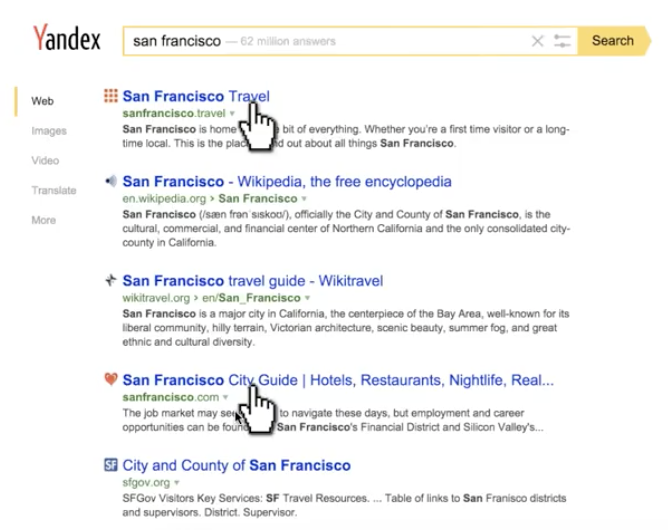
\includegraphics[scale=0.6]{figures/positionbased.png}
\end{figure}

Suppose we have the search results above and we observe the 2 clicks. How do we \textbf{model} this? \textbf{\textcolor{Maroon}{First}}, we randomly choose a result out of the 5, let's say we choose the 3rd one. We assume that the user first \textbf{\textcolor{Maroon}{examines}} the \textbf{snippet}. This is called the \textbf{\textcolor{Maroon}{probability of examination}}: $P_{exam}(3)$. This depends on the \textit{position}. \\
\\
\textbf{\textcolor{Maroon}{Secondly}}, if we like and think it is a good result for the \textbf{query}, we make another decision. Namely, we decide whether we are \textbf{\textcolor{Maroon}{attracted}} or not (by the snippet given our query). This is called \textbf{\textcolor{Maroon}{the probability of attractiveness}}: $P_{attr}(qd_3)$ (does not depend on examination). \\
\\
\textcolor{Maroon}{From lecture}: So see it as tossing 2 types of coins. First, you toss a coin from the \textbf{set of examination coins}, thereafter you toss a coin from the \textbf{set of attractive coins}. So you \textbf{\textcolor{Maroon}{click only}} if you \textbf{\textcolor{Maroon}{examine and find it attractive}}. Same applies for all 5 results $\{P_{exam}(1), P_{attr}(qd_1) \ldots P_{exam}(5), P_{attr}(qd_5)\}$.

\newpage

{\Large \textbf{Position-based model: \textcolor{MidnightBlue}{examination}}}:\\
{\large \textit{Terminology}}:
\begin{itemize}
    \setlength\itemsep{0em}
    \item \textbf{Examination} = reading a \textbf{\textcolor{Maroon}{snippet}}
    \item $E_r$ - binary random variable denoting examination of a snippet at rank $r$
\end{itemize}

{\large \textit{Position-based model (PBM)}}:
\begin{itemize}
    \setlength\itemsep{0em}
    \item Examination depends on rank: $P(E_r = 1) = \gamma_r$
\end{itemize}

So all \textcolor{Maroon}{probabilities of examination} will be replaced with $\gamma$, as following for example 5 results: $\{\gamma_1, P_{attr}(qd_1) \ldots \gamma_5, P_{attr}(qd_5)\}$. If the number of results is 100, then we would get 100 $\gamma$'s: $\{\gamma_1, \dots, \gamma_{100}\}$. \\
\\
\\
{\Large \textbf{Position-based model: \textcolor{MidnightBlue}{attractiveness}}}:\\
{\large \textit{Terminology}}:
\begin{itemize}
    \setlength\itemsep{0em}
    \item \textbf{Attractiveness} = a user wants to click on a document after examining it's \textbf{\textcolor{Maroon}{snippet}}
    \item $A_{qd}$ - binary random variable showing whethet document $d$ is attractive to a user, given query $q$
\end{itemize}

{\large \textit{Position-based model (PBM)}}:
\begin{itemize}
    \setlength\itemsep{0em}
    \item Attractive depends on a query-document pair: $P(A_{qd} = 1) = \alpha_{qd}$
\end{itemize} 

So all \textcolor{Maroon}{probabilities of attractiveness} will be replaced with $\alpha$, as following for example 5 documents: $\{\gamma_1, \alpha_{qd_1} \ldots \gamma_5, \alpha_{qd_5}\}$. If the number of documents is 100, then we would get 100 $\alpha$'s: $\{\alpha_{qd_1}, \dots, \alpha_{qd_{100}}\}$.\\
\\

\textbf{Position-based model: Summary}
\begin{itemize}
    \setlength\itemsep{0em}
    \item Probability of \textcolor{Maroon}{examination}: $P(E_{r_{d}} = 1) = \gamma_d$
    \item Probability of \textcolor{Maroon}{attractiveness}: $P(A_{qd} = 1) = \alpha_{qd}$
    \\
    \textcolor{red}{\rule{71ex}{1pt}}
    \item Probability of \textbf{\textcolor{Maroon}{click}}: $P(C_d = 1) = P(E_{r_{d}} = 1) \cdot P(A_{qd} = 1) = \gamma_d \cdot \alpha_{qd}$
\end{itemize}

\newpage
{\Large 1b). \textbf{Cascade model}: } 
\begin{enumerate}
    \setlength\itemsep{0em}
    \item Start from first document
    \item Examine documents one by one
    \item If click, then stop
    \item Otherwise, continue
\end{enumerate}

Again we \textcolor{Maroon}{click iff we examine and find it attractive}: $E_r = 1$ and $A_{d_{r}} = 1 \Leftrightarrow C_r = 1$.

The \textcolor{Maroon}{probability of attractiveness} stays the same, but there are some changes (see below): \\ 
\begin{minipage}{0.6\textwidth}
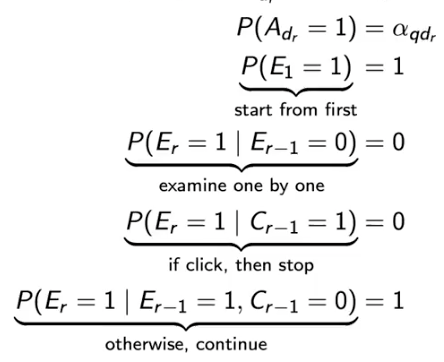
\includegraphics[scale=0.75]{figures/cascade.png}
\end{minipage}

\vspace{0.5cm}

{\Large \textbf{Basic click models summary}}: 
\begin{itemize}
    \setlength\itemsep{0em}
    \item Position-based model (PBM): \\
    + examination and attractiveness \\
    --  examination of a document at rank $r$ does not depend on examinations and clicks above $r$
    \item Cascade model (CM): \\
    + cascade dependency of examination at $r$ on examinations and clicks above $r$ \\
    -- only one click is allowed
\end{itemize}

\vspace{1cm}

{\huge 2). \textbf{Estimation} } \\
\\
\textbf{Parameter estimation}:
\begin{itemize}
    \setlength\itemsep{0em}
    \item Maximum likelihood estimation
    \item Expectation-maximization
    \begin{enumerate}
        \setlength\itemsep{0em}
        \item Set parameters to some initial values
        \item Repeat until convergence 
        \begin{itemize}
        \setlength\itemsep{0em}
            \item \textbf{E-step}: derive the expectation of the likelihood function
            \item \textbf{M-step}: maximize this expectation
        \end{itemize}
    \end{enumerate}
\end{itemize}

\vspace{0.5cm}

\textbf{EM update rules for PBM: \textcolor{Maroon}{attractiveness}} \\
\begin{minipage}{0.7\textwidth}
$ \alpha_{q d}^{(t+1)}=\frac{1}{\left|\mathcal{S}_{q d}\right|} \sum_{s \in \mathcal{S}_{q d}}\left(c_{d}^{(s)}+\left(1-c_{d}^{(s)}\right) \frac{\left(1-\gamma_{r}^{(t)}\right) \alpha_{q d}^{(t)}}{1-\gamma_{r}^{(t)} \alpha_{q d}^{(t)}}\right) $
\end{minipage}
\begin{minipage}{0.4\textwidth}
$t$: iteration \\
$S_{qd}$: search sessions iniated by query q and containing doc u \\
$c^{(s)}_d$: observed click on doc u in search sessions s
\end{minipage}

\vspace{0.5cm}

\textbf{EM update rules for PBM: \textcolor{Maroon}{examination}} \\
$ \gamma_{r}^{(t+1)}=\frac{1}{|\mathcal{S}|} \sum_{s \in \mathcal{S}}\left(c_{d}^{(s)}+\left(1-c_{d}^{(s)}\right)_{k} \frac{\gamma_{r}^{(t)}\left(1-\alpha_{q d}^{(t)}\right)}{1-\gamma_{r}^{(t)} \alpha_{q d}^{(t)}}\right) $

\vspace{0.5cm}

{\huge 3). \textbf{Applications} } \\
\\
\textbf{What can we get after estimation of a click model}?\\
\\
\begin{minipage}{0.5\textwidth}
\textcolor{Maroon}{Full probability} - probability that a user clicks on a document at rank $r$: $P(C_r = 1)$ \\
\\
\textcolor{Maroon}{Conditional probability} - probability that a user clicks on a document at rank r given previous clicks $P(C_r = 1 \mid C_1, \ldots, C_{r-1})$
\end{minipage}
\begin{minipage}{0.5\textwidth}
\;\;\;\; 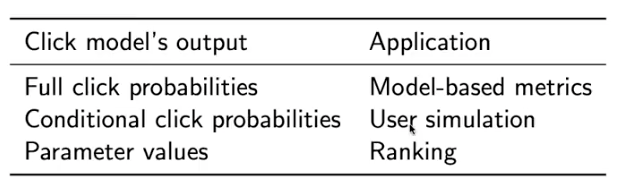
\includegraphics[scale=0.6]{figures/applications.png}
\end{minipage}

\vspace{0.65cm}

\textbf{Model-based metrics}: \\
\\
\begin{minipage}{0.5\textwidth}
Utitility-based metric: 
$$ \text { uMetric }=\sum_{r=1}^{n} P\left(C_{r}=1\right) \cdot U_{r}$$ 
Effort-based metric: 
$$\text { eMetric }=\sum_{r=1}^{n} P\left(S_{r}=1\right) \cdot F_{r}$$
\end{minipage}
\begin{minipage}{0.5\textwidth}
Expected reciprocal rank (ERR, second term last part from DBN): \\
\begin{align*}
    ERR &= \sum_r \frac{1}{r} \cdot P(S_r = 1) \\
    &= \sum_r \frac{1}{r} \cdot R_{qd_{r}} \cdot \prod^{r-1}_{i=1}(\gamma \cdot (1 - R_{qd_{i}})) 
\end{align*}
\end{minipage}

\vspace{0.25cm}
\begin{minipage}{0.5\textwidth}
Dynamic Bayesian network model (DBN) 
\begin{align*}
P\left(A_{r}=1\right) &=\alpha_{q d_{r}} \\
P\left(E_{1}=1\right) &=1 \\
P\left(E_{r}=1 \mid S_{r-1}=1\right) &=0 \\
P\left(E_{r}=1 \mid S_{r-1}=0\right) &=\gamma \\
P\left(S_{r}=1 \mid C_{r}=0\right) &=0 \\
P\left(S_{r}=1 \mid C_{r}=1\right) &=\sigma_{q d_{r}} \\
P\left(S_{r}=1\right) &=? 
\end{align*} 
\end{minipage}
\begin{minipage}{0.5\textwidth}
Dynamic Bayesian network model (DBN) 
\begin{align*}
P\left(S_{r}=1\right) &=P\left(S_{r}=1 \mid C_{r}=1\right) \cdot P\left(C_{r}=1\right) \\
&=\sigma_{q d_{r}} \cdot P\left(C_{r}=1\right) \\
&=\sigma_{q d_{r}} \cdot \alpha_{q d_{r}} \cdot P\left(E_{r}=1\right) \\
&=\sigma_{q d_{r}} \cdot \alpha_{q d_{r}} \cdot \prod_{i=1}^{r-1}\left(\gamma \cdot\left(1-\sigma_{q d_{i}} \cdot \alpha_{q d_{i}}\right)\right) \\
&=R_{q d_{r}} \cdot \prod_{i=1}^{r-1}\left(\gamma \cdot\left(1-R_{q d_{i}}\right)\right) \;\;(\textbf{ERR}).
\end{align*}
\end{minipage}

\newpage